% preliminaries %
\documentclass[11pt,letterpaper,onecolumn,twoside,openright,draft]{report}

%\usepackage{booktabs,fullpage,graphicx,showframe,todonotes}
\usepackage{booktabs,graphicx,setspace,showframe,todonotes}
% helpful: http://magic.aladdin.cs.cmu.edu/2005/08/25/setting-margin-in-latex/
\usepackage[dvips,letterpaper,margin=1in]{geometry}
% hyperref must be the last package
%\usepackage[backref,bookmarks,pdfpagemode=FullScreen,colorlinks=true]{hyperref}
\usepackage[bookmarks,pdfpagemode=FullScreen,colorlinks=true,pdfkeywords={PDF, LaTeX, hyperlinks, hyperref}]{hyperref}

% front matter %
\begin{document}
\title{Routes: A Multiagent Taxi Simulation}
\author{Tim Condit}
\date{\today}
\maketitle
\thispagestyle{empty}

\hyphenation{a-gents au-ton-o-mous com-pet-i-tive great-er Mul-ti-a-gent pa-ra-digms pick-up Py-thon slight-ly}

% use roman numerals for the front matter %
\pagestyle{headings}
\setcounter{page}{1}
\pagenumbering{roman}

\tableofcontents
\todo{add hyperlinks}
\listoffigures
\listoftables

% Break lines at sentences for version control sake.  Good stuff here:
% http://stackoverflow.com/questions/193298/best-practices-in-latex/196724#196724

% abstract (no page number) %
\begin{abstract}
Routes is a multiagent simulation of a Taxi service and its Fares.
All Taxis are created at the beginning of the simulation.
While the program is running, Fares enter the system at random times in random places.
Rather than requesting pickup through a central dispatch, the Fares broadcast their own locations locally, then regionally, and finally throughout the entire area, if needed.
Starting with the local region, all Taxis in a given range receive the Fare's pickup request and may decide to act on it, or they may ignore it, depending on their circumstances and the type of simulation being run.

Functional transit maps are generated in real-time from Census Bureau data that includes the entire United States of America and territories.
The size of the transit map, and hence the simulation's range can be as small as a single area code, up to an entire county.
The data that is downloaded to generate the transit map is processed locally the first time it's used, and cached to save time (and bandwidth) for subsequent runs.

\todo{Add something here about the transit map being a big network graph. Can probably pull something directly out of the full text.}

There are three different negotiation protocols - first-in, first-out, closest Fare, and mixed mode.
There are two simulation types - cooperative and competitive.
They are combined for a total of six different simulations.
\end{abstract}

% switch to Arabic numbers for the body - and restart the page count %
\pagenumbering{arabic}
\setcounter{page}{2}

% introduction %
\chapter{Introduction}

Routes is a simulation of a taxi service.

Taxi services have operated the same way for many years.
Wherever they operate, it is common to get a ride by flagging down a taxi from the side of the road.
Most taxi companies also have dispatchers who will arrange pickup at a later time.\footnote{A notable exception is New York City, where a fare cannot be prearranged.
Only for-hire vehicles such as livery cars or limousines may prearrange pickup.

{\hyperlink{http://www.nyc.gov/html/tlc/downloads/pdf/fhv_base_fact_sheet.pdf}{Understanding the For-Hire Vehicle Industry}}
\hyperlink{http://www.nyc.gov/html/tlc/html/passenger/faq_pass.shtml\#14} {How can I pre-arrange a trip in a Yellow Cab?}}

\todo{the hyperlinks below are broken}

Taxi services are subject to extensive regulation, and are in some ways similar to a public utility.\footnote{This site documents legal actions and taxi regulations all over the world: {\hyperlink{http://www.taxi-library.org/regulation.htm}{Regulation of Taxicabs}}}

For example, the rates charged by municipal taxi services are often set by the city or county in which the taxis operate.
This means that among other things, they cannot compete on price, since they are all forced to charge the same rates for the same trips.

The simulations presented in this paper have none of these restrictions.
They are closer to a loose confederation of independent drivers than to a highly regulated municipal utility.
They are missing a couple key features of terrestrial taxis.
First, they cannot be flagged down for a pickup.
If they are not on their way to pick up a Fare, or driving the Fare to it's destination, they are not moving.
Second, they do not have a dispatcher.
This is a key component.
They operate in a distributed fashion, with the Fare initiating contact with the Taxis directly, and - in the cooperative simulations anyway - the Taxis communicating amongst themselves about which one will pick up a given Fare.

They ask and try to answer the following questions:
\begin{itemize}
  \item{Is an autonomous, distributed Taxi system technically feasible, at least conceptually?
    How would it work?}
  \item{How would the dynamic change when Agents (Fares and Taxis) communicate with each other directly?}
  \item{Would a Fare be willing to wait a little longer for a better price?
    (This implies that the now hidden cost of driving to a Fare is explicitly included in the cost of the fare, since without the cost of making the pickup there is no chance to earn the revenue of the trip.)}
  \item{What would happen if both the Taxi and the Fare had to be satisfied that the trip was worthwhile?
    And what if as a result of these constraints, some Fares get no service?}
  \item{What would happen if Taxis had to compete for Fares with their fellows?
    Would this improve service for all?
    Or would a cooperative model work better at the team or organization level?}
  \item{What would happen if two teams of Taxis competed with each other?
    In other words, the Taxis of two teams A and B would coordinate Fare pickup amongst themselves, but they’d be competing with the other team, and will lose some of the Fares.
    Would the results be much different at the system level than what happens when it’s "every man for himself"?}
\end{itemize}

But mostly this is a paper that explores the use of autonomous agents.
They are characterized this way in \cite{roozemond2000act}, in a section called "What are intelligent agents?":

\quote{Multi-Agent Systems can be characterised by the interaction of many agents trying to solve a variety of problems in a cooperative fashion.
Besides AI, intelligent agents should have some additional attributes to solve problems by itself in real-time; understand information; have goals and intentions; draw distinctions between situations; generalise; synthesise new concepts and/or ideas; model the world they operate in and plan and predict consequences of actions and evaluate alternatives.
The problem solving component of an intelligent agent can be a rule-based system but can also be a neural network or a fuzzy expert system.}

The Agents in this series of simulations meet most of these criteria.
In half the simulations the Agents work together in a cooperative fashion - in the other half, they are competitive; they are able to solve problems by themselves in real-time; they understand Fare requests for pickup (information); they have goals and intentions; and they draw distinctions between situations to determine whether to reserve (or compete for) a particular Fare.
They don't do much generalizing or synthesizing of new concepts, but they do model the world in which they operate, and predict the consequences of their actions and act accordingly.

The Agents are Taxis and Fares, but in another context they may have been viruses and antibodies, or cowboys and indians.
Both may draw attention away from the simulations, in different directions: viruses and antibodies may be too complex, and cowboys and indians may be too simple.
Taxi services in the real world do not have many competitive freedoms.
The main goal of all the regulation seems to be about providing a reliable service with predictable prices.
Those are fine goals, but the simulations in this paper step outside those boundaries, and explore what would happen if things were allowed to evolve differently.

The higher priority for this paper was flexibility in designing the negotiation protocols and simulations.
Taxis and Fares are not the only choice of autonomous agents to study, but they serve the purpose well.
% that last bit sounds like it belongs in the conclusion

\section{Definition of Terms}
The following terms are used throughout the paper:
\todo{add the definitions!}

\section{Organization}
The rest of the paper consists of the following sections:

\begin{itemize}
  \item{RELATED WORK is a review of the literature.
    Research on taxis as autonomous agents is scarce, but there are traffic and road network simulations that come at the issue from a different direction.
    Instead of looking at a system of mobile agents, stationary agents at traffic lights provide information for improving the flow of traffic or routing around accidents and congestion.
    The Belief-Desire-Intention model of intelligent agents is reviewed, and the Routes agents are categorized within a framework for organizing classes of multi-agent systems for transport logistics.
    (This is not directly related, unless people are considered goods to transport, but it clarifies a few things about the agents nevertheless.)}
  \item{IMPLEMENTATION describes the Taxis and Fares in \linebreak greater detail.
    It explains the grids and graphs that make up the Agent's world, and the network traversal algorithms that calculate routes around the different regions.
    It expands on the negotiation protocols and simulation types.
    Finally it describes the simulation software that drives the whole process, the extensive run-time configuration options, and the interactive environment within which the simulations are executed.}
  \item{RESULTS tells the story of the simulations.
    Individual Agents have autonomy during runtime, but from a simulation point of view, the agents are part of larger system.
    Several simulations are run and their data plotted and reported here.}
  \item{CONCLUSION brings things to a close, and enumerates a number of possible future enhancements.
    There are a number of ways this program could be expanded upon, and the source code will be freely available upon acceptance of this report.}
  \item{APPENDIX A: USING TIGER/LINE DATA describes how raw data from the U.S. Census Bureau, representing roads throughout the United States and it's territories, is converted in real-time into line segments, and how those line segments are knit together to make network graphs upon which the simulations are run.}
  \item{APPENDIX B: ANNOTATED CONFIG FILES enumerates the large collection of both agent and graph data that can be customized at run-time, including full annotations about each setting.}
  \item{APPENDIX C: LIST OF OPEN SOURCE SOFTWARE\ldots}
  \item{APPENDIX D: SOURCE CODE\ldots}
  \item{APPENDIX E: TRANSCRIPT OF INTERACTIVE SESSION\ldots}
\end{itemize}

\todo{existence proof only: get rid of them}
\cite{davidsson2005aab}
\cite{yokoo1999}

% use this?
% cite: http://en.wikipedia.org/wiki/Multi-agent_system, accessed 1/11/2009
%
% Autonomy: the agents are at least partially autonomous
% Local views: no agent has a full global view of the system, or the system is too complex for an agent to make practical use of such knowledge
% Decentralization: there is no one controlling agent (or the system is effectively reduced to a monolithic system)


% related work %
\chapter{RelatedWork}
\section{Introduction}
In this section I examine features found in other multiagent systems to see how they contrast with my system.
The focus in the applied literature is on traffic and road network simulations.
Two of the papers describe centralized versus distributed simulation systems\cite{france2003mso,hernandez2001}.
One of them includes an implemented and installed system, while the other is evaluated using a mathematical formula describing variable levels of traffic congestion.
Aside from the fact that one is applied and the other more theoretical, their approaches are different enough to make a useful comparison.
Then I investigate an uncertainty management framework for understanding relationships between agents in a multiagent sytem\cite{wu2003umf}.
This paper uses the Belief-Desire-Intention (BDI) agent model to formulate a response to received inputs.
The last paper is a review of multi-agent systems (MAS) used for transport logistics\cite{davidsson2005aab}.
My software is classified according to this scheme.

\section{Centralized and Distributed Multiagent Traffic Systems}
Reviewing decision support systems (DSS) for use in traffic management.

\subsection{Regional Agent Coordination with TRYS and TRYSA$_{2}$}
Hern\'{a}ndez et al.\cite{hernandez2001} describes a pair of closely related intelligent traffic management systems (ITMS).
The TRYS\footnote{The acronym is not identified in the paper.} system is implemented and in use in Barcelona, Spain.
TRYSA$_{2}$\footnote{TRYS Autonomous Agents} is developed only to the prototype level at time of publication, but was validated with the same data as the first system.
Both systems partition a highly congested local traffic network into a series of overlapping problem areas, which are monitored by traffic control agents.
These agents collect data via vehicle detectors and telemetered sensors ("loop detectors").
The raw data is used to generate traffic control plans, but they are advisory only.
A human operator makes the final decision on how the plans are used.

These systems are fundamentally different from the approach I have taken for several reasons.
The first, and most important difference is that these are not simulations.
Second, they are open systems in the sense that the outputs are "processed" by a traffic engineer, as opposed to a closed and terminal system, where the final result is the end of the simulation, rather than inputs to an "offline" system.
Finally, the focus here is on the traffic network exclusively, with zero representation of the users of the network, i.e. drivers and passengers.
Regardless, there are some interesting contrasts.

TRYS is a centralized multiagent system.
It operates on inputs from more than 300 telemetered sensors and feed data to the local traffic control center.
The goal of this system is to provide traffic engineers with alternatives for traffic light coordination.
It is more coordinated than autonomous; each agent has to take its neighbor's state into account when designing their traffic control plan.
Imagine a series of traffic lights that are not coordinated with each other in some way.
The individual agents would still generate plans based on the inputs they are receiving.
You might reasonably expect there to be some kind of emergent or spontaneous coordination, but it would most likely not be globally consistent.
Therefore, the local control plans generated by the first-level agents are sent to a special coordinator agent responsible for integrating local control proposals into a coherent global signal plan for the whole traffic network.
The coordinator resolves any conflicts between the local control proposals then sends the globally consistent local signal plans back to the traffic agents.
% and also to the traffic engineer?

An interesting feature of this system is the way in which the agents decide on which traffic control plans to forward to the coordinator.
The agents are provided with data about the traffic congestion ("demand knowledge") and some expectation of how different actions will affect the flow
of traffic ("expected redistribution").
Given these pieces of information, they run a macrosimulation to decide if there will be an adequate decrease in the excess flow.
They forward the plan to the coordinator if appropriate, and reject it otherwise.

TRYSA$_{2}$ is a reformulation of TRYS using autonomous agents.
Whereas TRYS uses a more linear form of communication between the traffic control agents and the coordinator, agents in TRYSA$_{2}$ communicate with one another directly, eliminating the need for a coordinator agent.
See figure~\ref{fig:TRYS-and-TRYSA2} on page~\pageref{fig:TRYS-and-TRYSA2}.

\begin{figure}[h]
  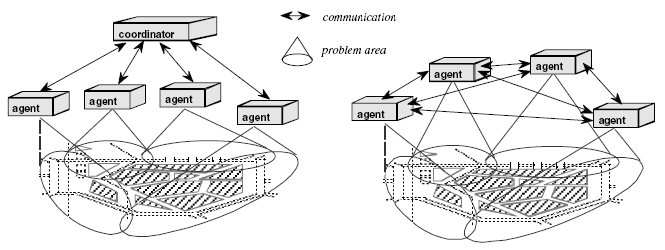
\includegraphics{figures/TRYS-and-TRYSA2.PNG}
  \caption{Centralized (TRYS) and decentralized coordination (TRYSA$_{2}$).}
  \label{fig:TRYS-and-TRYSA2}
\end{figure}

The partitioning of the road network into problem areas is slightly different from that in TRYS, but problem detection, diagnosis and selection of control plans are similar.
Each traffic control agent in TRYSA$_{2}$ maintains its own set of alternative traffic control plans, along with expected reductions in local traffic excesses associated with each of the plans.
This is called the plan's local utility.

This is where things get interesting in TRYSA$_{2}$.
The autonomous agents use a strategy called structural cooperation\cite{ossowski1999}, whereby they take their own utility and the effects of their acquaintances' control plans on their own utiltiy into consideration when deciding what to do.
In short, the agents are no longer fully autonomous.

The paper describes the situation and the response to it this way:

\quote{There is a conflict of interest respecting the way in which local signal plans are adapted.
The essential idea is that the more autonomous an agent is (i.e. the less its local utility can be influenced by others), the more weight will have its opinion respecting which local plans to modify and how to adapt them.
Still, sometimes the resulting basic coordination does not lead to globally optimal control plans, so the system designer can issue rights or prohibitions for some agents to use control devices in certain ways.
By this, he modifies the degree of autonomy of some agents, biasing the outcome of coordination (i.e. the resulting global signal plan) in a desired direction.}

The agents choose local signal plans, but they still need to coordinate with one another to settle on a globally consistent signal plan.
This is similar to the task of the coordinator agent in TRYS.
To do this the agents use a distributed constraint optimization protocol\footnote{The original basis for my work, although it did not make it into the final product.} that implements weak commitment search\cite{yokoo1999}.
\todo{This is referenced in Hernandez, but not in this paper.
I should probably dig up the reference anyway.}

This is a three-stage process.
In stage 1 the local control agents repeatedly exchange utility information to find sets of globally compatible alternative signal plans.
Stage 2 starts when one of the agents detects the completion of stage 1.
This agent computes approximate probabilities that each of the chosen sets of local signal plans would be enacted, and from that attempts to maximize the product of the local agent utilities.
In other words, lower quality plans are dropped from consideration.
In stage 3 a set of local signal plans are selected by lottery, and the results are shared with all agents.
This concludes the work of the autonomous agents in TRYSA$_{2}$.
\todo{need something here to break up the flow and signal that we're starting a new section}
At this stage in both systems the selected control plans are ready for review by the traffic engineer.

\subsection{Comparison with Routes}
There are several ways in which these systems differ from mine: they are decision support systems, whereas mine are simulations; they are traffic network-oriented, whereas mine are agent-oriented; one of them is in production use and the other is a prototype, whereas mine is fully implemented but on a smaller scale.
On the other hand, this paper provides something that was hard to come by: a look at similar systems implemented on both a centralized and distributed paradigms.
That and the fact that it was a multiagent traffic management study, made it a useful choice.

One superficial similarity of TRYS and TRYSA$_{2}$ with my system is in the representation of the physical structure of the traffic network.
It uses a declarative description of the network as a graph with nodes and links together with abstraction functions associated to components, described here as "static information about the topological structure of the problem area".
\todo{need something here to break up the flow and signal that we're starting a new section}
Next we look at another multiagent system for optimizing an urban traffic network.

\subsection{Local and Global Agent Coordination}
This paper\cite{france2003mso} is similar in many ways to the previous one.
It is another centralized multiagent system for traffic management that uses local traffic agents and one or more coordinator agents.
But this paper uses traffic intersections as the problem area, rather than larger regions, and builds a hierarchical structure involving other types of coordinating agents as well.

The first goal of this system is to design a traffic network that operates in real-time and takes into account that traffic lights essentially operate in an infinite loop, or as a non-finite process.
The second goal is to handle dynamically occuring events such as traffic accidents or roadway congestion in a coordinated fashion.
With autonomous agents at each intersection, agents at neighboring intersections are unaware of traffic events occuring elsewhere, leading to detrimental traffic flow.
For instance, this system would allow traffic to continue toward a blocked intersection in the case of an accident.
\todo{Does this sentence "With agents at each intersection\ldots" break the flow?}
The final goal is to balance local and global concerns with respect to traffic movement.
Local traffic agents (LTA) will typically have many alternative plans available, but several of them are incompatible with the global goals of traffic management.
A major task is for the coordinator traffic agents (CTA) to quickly figure out which ones to drop from consideration.
This was addressed in Hern\'{a}ndez, but real-time performance data was not provided.

The LTAs and the CTAs behave almost identically to the analogous agents in TRYS (see figure~\ref{fig:LTAs-and-CTA} on page~\pageref{fig:LTAs-and-CTA}).
But this is a more general system that was not designed for a specific traffic network.
It may be used on larger roadways where multiple CTAs are needed.
In this case, a Global Traffic Agent (GTA) is added to the hierarchy, and all CTAs report to it.
The LTAs do not communicate with each other, but only with their assigned CTAs.
Likewise, if a traffic network is large enough that a GTA is needed, it is subdivided into regions controlled by a single CTA, with a top-level GTA linking the CTAs together.
The final piece of the agent hierarchy is the Information Traffic Agent (ITA).
As the name suggests, the ITA stores and distributes all information detailing the state of each intersection.
Each LTA and CTA communicate directly with the ITA, but it does not process any data.
Its only purpose it to store traffic data and provide immediate feedback to the other agents.

\begin{figure}[h]
  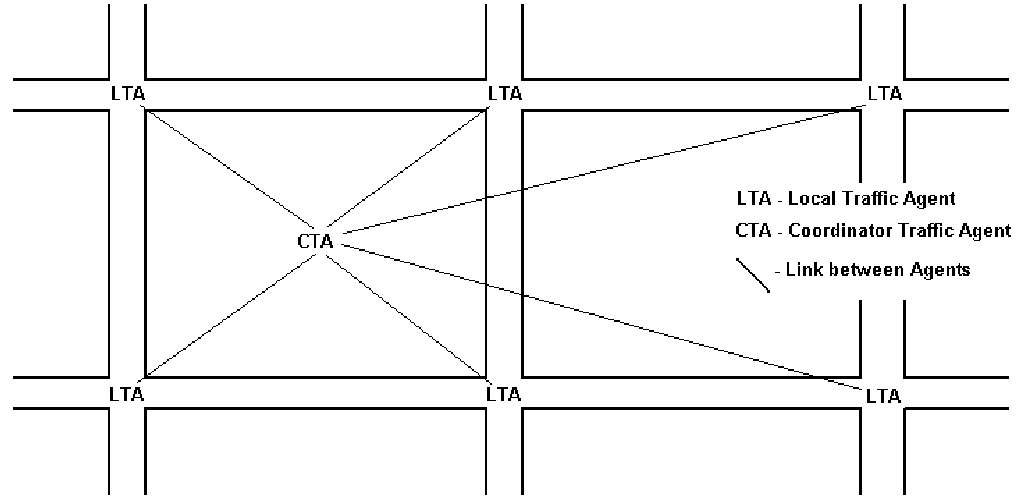
\includegraphics{figures/LTAs-and-CTA.PNG}
  \caption{Layout of Local and Coordinator Traffic Agents.}
  \label{fig:LTAs-and-CTA}
\end{figure}

\todo{use a subfloat for the map and graph side-by-side images (whenever I get around to doing it)}

When deciding on a traffic light pattern, most communication takes place between the LTAs and the CTAs, with the ITAs providing stored data as necessary.
In order for the CTA to calculate a global optimum for a given intersection, it must collect data from all neighbors of that intersection's LTA.
The ITA provides data about traffic levels, congestion, accidents, etc. at each of the intersections requested by the CTA.
The CTA calculates a traffic light pattern and compares it to that proposed by the LTA.
\todo{Do I need something here about the LTAs generating their own proposed traffic light pattern for review by the CTA?}
If there is a significant difference between them, a balance between the local and global optimums must be reached, and communicated to the LTA\footnote{The authors do not describe how they negotiate this balance.}.
Traffic sensors provide data to the ITAs.
Collected data includes the current state of each traffic light, the direction of traffic movement, e.g. North heading North or West, or South going East, and the time remaining for the light in its current state.
The LTAs include an expert system that uses this data to calculate a locally optimal light pattern, without regard to other intersections.
Following this the LTA sends a message to the CTA, which may adjust the LTA's light pattern, based on the recommendation of its own expert system, to accomodate the needs of the global network.

The communication protocols described earlier are also used by the CTAs to send real-time updates of events occuring within the system.
The events described in this paper are traffic accidents and roadway congestion.
Most events affect only a small number of LTAs, and only directly affected agents are notified of the events.

An agent is considered affected by a traffic accident if the accident occurs at a neighboring intersection, a connecting roadway, or within agent's intersection.
When an LTA is notified by the CTA that it is affected by a traffic accident\footnote{The CTA receives the notification manually from a human operator. In other words, this part of the application was not implemented at the time of publication.}, it overrides the state of the traffic light pattern provided by the CTA, for the duration of the event.
Essentially, the agent regains its autonomy, and decides for itself what action to take during the disruption.
Reading between the lines, it seems that the LTA recalculates its own local traffic light pattern, and uses that until further notice from the CTA.
When the LTA is notified that the event has passed, the light returns to standard operation.

In the case of traffic congestion at a neighboring intersection, the CTA will look for an alternate route to redirect incoming traffic.
If none is found, the soon-to-be affected LTA is sent the red signal, effectively halting incoming traffic.
If an alternate is found, the CTA will send a message to the LTA that is experiencing the congestion.
The LTA will again override the traffic light pattern, but this time it is only for a single cycle of the traffic light pattern, after which it reverts to the pattern provided by the CTA.
The CTA has the option to recall the pattern event, leaving the overridden pattern active at the LTA.
This cycle could then be repeated by the CTA for as long as necessary, based on updated sensor data.

\subsection{Comparison with Routes}
By way of comparison with my work, this system is traffic network-oriented rather than agent-oriented.
It is also more hierarchical, with little autonomy for agents.
The LTAs are not allowed to communicate directly with one another.
In larger systems with multiple CTAs, they are not allowed to communicate with one another either.
On the other hand, this is an applied approach at solving a specific problem, rather than exploring the nature of agent-based simulations.
The first priority here is to find something that works, whereas my system is geared toward exploration, with optimality a nice side-effect, but not the primary goal.

\section{Cooperative and Competitive Multiagent Systems}
Here we investigate coordination, cooperation and competition among software agents.

\subsection{Extending the Belief-Desire-Intention Model}
The Wu paper\cite{wu2003umf} develops a system for identifying agent uncertainty in relation to other agents in a MAS.
They build upon the existing BDI (belief-desire-intention) agent model, adding
a new attribute, KB (knowledge base), and attribute properties\todo{should I mention in a footnote that I use the terms properties and "state modifiers" interchangably?} public, private and protected.
This enhanced model is intended for use within a decision support system.
It gives individual agents a better understanding of their position relative to other agents.
This should allow the agents to make better informed decisions.
BDI is described here to put it into context as part of the overall definition of the uncertainty management framework.

\emph{Belief} is the information available to an agent about the state of the environment.
It is a frequently updated attribute described by the function \[\wp\emph{(Belief)}\times \emph{P}\to\wp\emph{(Belief)}\] where \emph{P} is the agent's current precept and current beliefs.
\emph{Desire} is the set of options an agent can use to achieve its intentions.
It is derived from the agent's belief and intentions and is described as \[\wp\emph{(Belief)}\times \wp\emph{(Intentions)}\to\wp\emph{(Desire)}\]
The agent's \emph{intention} is simply what it wants to do or accomplish\footnote{This paper does not include a precise definition of intention}.
The new piece, the \emph{knowledge base}, expands on the concept of the agent's intention.
It is a database of related information on a particular subject that describes how to do a certain task.
The four attributes in the extended BDI agent model are not sufficient to model an agent's relationships with its cohorts.
The authors add three state modifiers -- public, private and protected -- to each of these attributes.
Public properties are visible to all, while private properties are visible only to the agent.
An attribute with protected properties, on the other hand, is one where its probability distribution is visible to others.

Now we can describe the uncertainty management framework with respect to cooperation, coordination, and competition, and again, it starts with definitions.
A cooperating agent in this system is defined one that reveals its beliefs, desires, intentions and knowledge base to others.
In addition, all cooperating agents must have the same goal.
Coordination is defined as revealing an agent's intentions and knowledge base to others, but the agents have differing goals.
In loose competition an agent's goal is revealed, but not his knowledge base.
In strict competition an agent reveals neither his goal or knowledge base.
In either of the latter cases, the agent's beliefs and desires may be public, private or protected (this is a function of the how much uncertainty exists in the system) and agents may have the same or different goals as others.

Taken together, the attributes plus properties lead to a series of actionable decision-making states.
The variable attributes are beliefs and desires.
The intentions may be public or private for any of these agent interactions, but it does not affect the decision making classification.
In every case, the agent's KB is private.
\todo{need something here to break up the flow and signal that we're starting a new section}

With \emph{decision making under certainty}, between any pair of agents, both agents beliefs and desires are public and readable by the other.
In \emph{decision making under risk}, both agents' beliefs and desires are protected, so their exact state is not known, but their probability distributions are available, which should allow the agents to make some reasonable predictions about each other's expected actions.
Finally, with \emph{decision making under uncertainty}, neither agent knows anything about the other agent's beliefs or desires.
Data collection is entirely speculative. See figure~\ref{fig:uncertainty-management} on page~\pageref{fig:uncertainty-management} for a summary.

\begin{figure}[h]
  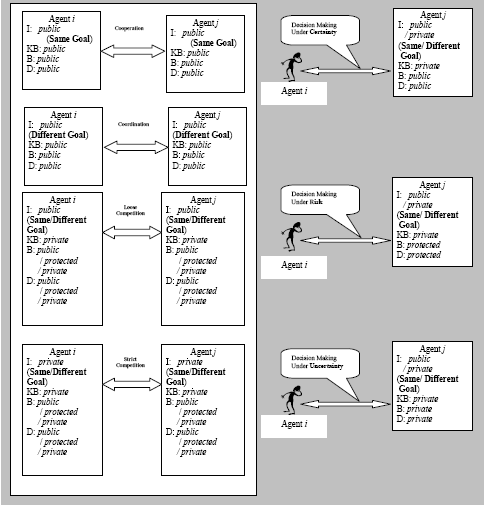
\includegraphics{figures/uncertainty-management}
  \caption{Modeling agents' interactions using BDI \& three types of decision making.}
  \label{fig:uncertainty-management}
\end{figure}

\subsection{Comparison with Routes}
By way of comparison, in my cooperative simulations, the Taxis communicate with the Fares soon after the initial pickup request is made.
This is similar in practice to decision making under certainty, as both kinds of agents (or maybe more accurately, the agents with different goals) are communicating openly with one another.
The Fare receives an acknowledgment before pickup, and the other Taxis are notified that a particular Fare is no longer eligible.

In my competitive simulations, the Taxis make decisions under something approximating risk in the Wu model.
Whereas their system allows agents to share probability data with one another, in my system there are only a few decisions that a Taxi is likely to make, and they are made in private.
When any two or more agents (Taxis) compete for a Fare, there will be exactly one winner, and all other competitors will lose that Fare.
But until a Taxi announces publicly that he has reached the Fare first, all movement is private.
Note also that the Fares do not communicate with one another, but only because it adds nothing to the simulation as designed.
There are certainly enhancements where communication between potential Fares would raise their attractiveness to Taxis, thereby increasing their fitness for pickup, resulting in better (faster) responses from the Taxis.

One additional note: although I have no plans currently to include it in this paper, I have run some Taxi "team" simulations with the current system.
The Taxis in these simulations behave similarly to agents making decisions under risk.
For any two agents, there are two possible scenarios: they are cooperating, meaning they are on the same "team", or they are coordinating, meaning they are on different teams.
Both scenarios assume a SimType of cooperative.
A SimType of competitive does not make much sense here, since the Taxis would be competing with their teammates and with the Taxis on the other team or teams.
The whole program would have to be modified to make a useful team competition.

\subsection{Putting This Project Into Context}
The last paper in this series is a review of agent-based approaches to transportation and traffic management.
The authors have developed a classification system that is used to organize the large number of papers in the review.
While the focus is primarily on logistics, I classify my work as it fits into their system.

The article defines the concepts of logistics in some depth.
Here they are talking about transport logistics, or the movement of goods from one place to another, often through multiple means, for example rail to ship to rail.
The most succint definition of logistics that I found is "Logistics means having the right thing, at the right place, at the right time."\footnote{http://www.logisticsworld.com/logistics.htm}
My system is neither a traffic management nor a logistics flow model, unless you consider the Fares as product to be moved from place to place.
Nevertheless, there are parallels and the classification is enlightening.

The evaluation framework consists of several pieces.
The full list is shown in table~\ref{tab:transport-logistics-eval-framework}.
Most of them will be clear from the context, but I will expand on some of them.
Under \emph{Approach}$\to$\emph{Usage} are the categories Automation System and Decision support system (DSS).
This is a recurring theme in multiagent logistics and traffic management systems.
This is the first time I've seen the term automation system used to describe the alternative to DSS.
It is defined as "having a self-acting mechanism that performs a required act at a predetermined time or in response to certain conditions."
That's a reasonable, if general, description of my system.
\emph{Approach}$\to$\emph{MAS structure} corresponds to the interactions of the agents, whether it is static, meaning the agents have the same roles throughout the simulation, or dynamic, where roles may change over time.
\emph{Approach}$\to$\emph{Agent attitude} splits the agent interactions into two categories.
All agents are classified as either benevolent (cooperative) or selfish (competitive).
They do not make the distinction between cooperative and coordinative agents.
In any event, my system includes both cooperative and competitive agents.

\todo{Drop this paragraph?}
The article mentions Multi Agent Based Simulations (MABS), a term that simply means that the agents in the simulation may have different roles, e.g. a company, a truck, a customer, etc.
We've seen similar examples of this with the LTAs and CTAs in the France paper.
My agents are designed similarly.
But this is the first term I've found to describe agent partitioning based on role.

The Taxis and Fares system is described according to the Davidsson classification scheme in table~\ref{tab:classifying-taxis-and-fares-sim}.
All six simulation types are listed.
Most of the data in the table is identical across all my simulations.
This is maybe not surprising, since they are all part of the same system.
The only difference is between the cooperative and competitive NPs: the cooperative simtypes are described as benevolent, and competitive as selfish.

% Table generated by Excel2LaTeX from sheet 'txport-logistics-eval-framework'
\begin{table}[htbp]
  \centering
    \begin{tabular}{|l|p{0.25\textwidth}|p{0.37\textwidth}|}
    \addlinespace
    \hline
    %\toprule
          & \textbf{Aspect} & \textbf{Categories} \\
    %midrule
    \hline
    \hline
    \textbf{Problem Description} & Domain & 1. Transport \\
          &       & 2. Traffic \\
          &       & 3. Terminal \\
          %\hline
          \cline{2-3}
          & Transport mode & 1. Air \\
          &       & 2. Rail \\
          &       & 3. Road \\
          &       & 4. Sea \\
          &       & 5. Intermodal \\
          %\hline
          \cline{2-3}
          & Time horizon & 1. Operational \\
          &       & 2. Tactical \\
          &       & 3. Strategical \\
          \hline
          %\cline{2-3}
    \textbf{Approach} & Usage & 1. Automation system \\
          &       & 2. Decision support system \\
          %\hline
          \cline{2-3}
          & Control & 1. Centralized \\
          &       & 2. Distributed \\
          %\hline
          \cline{2-3}
          & MAS Structure & 1. Static \\
          &       & 2. Dynamic \\
          %\hline
          \cline{2-3}
          & Agent attitude & 1. Benevolent \\
          &       & 2. Selfish \\
          %\hline
          \cline{2-3}
          & Agent architecture & 1. Reactive \\
          &       & 2. Deliberative \\
          &       & 3. Hybrid \\
          \hline
          %\cline{2-3}
    \textbf{Results} & Maturity & 1. Conceptual proposal \\
          &       & 2. Simulation experiment \\
          &       &   2.1. artificial data \\
          &       &     2.1.1. limited/partial \\
          &       &     2.1.2. full scale \\
          &       &   2.2. real data \\
          &       &     2.2.1. limited/partial \\
          &       &     2.2.2. full scale \\
          &       & 3. Field experiment \\
          &       &   3.1. limited/partial \\
          &       &   3.2. full scale \\
          &       & 4. Deployed system \\
          %\hline
          \cline{2-3}
          & Eval comparison & 1. None \\
          &       & 2. Qualitative \\
          &       & 3. Quantitative \\
    %\bottomrule
    \hline
    \end{tabular}%
  \caption{Summary of transportation logistics evaluation framework}
  \label{tab:transport-logistics-eval-framework}%
\end{table}%

% Table generated by Excel2LaTeX from sheet 'classifying-taxis-and-fares-sim'
\begin{table}[htbp]
  \centering
    \begin{tabular}{|l|p{0.26\textwidth}|p{0.18\textwidth}|p{0.18\textwidth}|p{0.18\textwidth}|}
    %\begin{tabular}{|l|l|l|l|l|}
    \addlinespace
    \hline
    %\toprule
          %&       & \textbf{Cooperative/FIFO} & \textbf{Cooperative/CF} & \textbf{Cooperative/MM} \\
          &       & \emph{\textbf{Coop/FIFO}} & \emph{\textbf{Coop/CF}} & \emph{\textbf{Coop/MM}} \\
          \hline
          \hline
    %\midrule
    \textbf{Problem Description} & Domain & Traffic & Traffic & Traffic \\
          \cline{2-5}
          & Transport mode & Road  & Road  & Road \\
          \cline{2-5}
          & Time horizon & Operational & Operational & Operational \\
          \hline
    \textbf{Approach} & Usage & Automation system & Automation system & Automation system \\
          \cline{2-5}
          & Control type & Distributed & Distributed & Distributed \\
          \cline{2-5}
          & MAS structure & Static & Static & Static \\
          \cline{2-5}
          & Agent attitude & Benevolent & Benevolent & Benevolent \\
          \cline{2-5}
          & Agent architecture & Reactive & Reactive & Reactive \\
          \hline
    \textbf{Results} & Maturity & 2.2.1 & 2.2.1 & 2.2.1 \\
          \cline{2-5}
          & Eval comparison & Qualitative & Qualitative & Qualitative \\
          \hline
          \hline
          \cline{2-5}
          %\\[3pt]
          %\vspace{4.8mm}
%    \end{tabular}%
%  \caption{Classifying the Taxis and Fares simulation, part 1}
%\end{table}%
%
%\begin{table}[htbp]
%  \centering
%    %\begin{tabular}{|l|p{0.16\textwidth}|p{0.16\textwidth}|p{0.16\textwidth}|p{0.16\textwidth}|}
%    \begin{tabular}{|l|l|l|l|l|}
%    \addlinespace
%    \hline
%    %\toprule
%          %&       & \textbf{Competitive/FIFO} & \textbf{Competitive/CF} & \textbf{Competitive/MM} \\
          &       & \emph{\textbf{Comp/FIFO}} & \emph{\textbf{Comp/CF}} & \emph{\textbf{Comp/MM}} \\
          \hline
          \hline
    \textbf{Problem Description} & Domain & Traffic & Traffic & Traffic \\
          \cline{2-5}
          & Transport mode & Road  & Road  & Road \\
          \cline{2-5}
          & Time horizon & Operational & Operational & Operational \\
          \hline
    \textbf{Approach} & Usage & Automation system & Automation system & Automation system \\
          \cline{2-5}
          & Control type & Distributed & Distributed & Distributed \\
          \cline{2-5}
          & MAS structure & Static & Static & Static \\
          \cline{2-5}
          & Agent attitude & Selfish & Selfish & Selfish \\
          \cline{2-5}
          & Agent architecture & Reactive & Reactive & Reactive \\
          \hline
    \textbf{Results} & Maturity & 2.2.1 & 2.2.1 & 2.2.1 \\
          \cline{2-5}
          & Eval comparison & Qualitative & Qualitative & Qualitative \\
    %\bottomrule
    \hline
    \end{tabular}%
  \caption{Classifying the Taxis and Fares simulation}
  \label{tab:classifying-taxis-and-fares-sim}%
\end{table}%

\todo{old comment: Modi - ADOPT: Asynchronous Distributed Constraint Optimization with Quality Guarantees}
\todo{old comment: Mailler - Solving Distributed Constraint Optimization Problems Using Cooperative Mediation}


% implementation %
\chapter{Implementation}
\todo{Add something in here about Python duck-typing in the grid and graph classes.
They are considered something like equivalent because they have the same set of methods.
There's no need to mess around with interfaces or extending the same base class.
(Use that too. That's good.)}
\section{Grids and Graphs}
\todo{Nothing here yet.}

\todo{Among other things, this is where the side-by-side map images will go.}

\section{SimPy Resource Types: Resources, Levels and Stores}
The three types of SimPy resources available for working with the actors in a simulation are Resources, Levels and Stores.
Depending on the complexity of the simulation, you may use one or more of them, but any individual piece is modeled using only one.
I describe them here, and then explain how they are used in Routes.

The first type, a Resource, is useful if you have multiple identical tasks that are modeled as SimPy objects, and require one or more discrete elements.
The example most often given here is waiting in line at a bank.
The tellers are the required elements (a SimPy Resource), and the customers waiting to perform some task (also a Resource) wait in a shared line for a teller to become available.
The waiting customers are stored in a wait queue, while the customers who are at the teller stations are stored in an active queue.

The second resource type is the Level.
It is used when you want to model something of a more continuous nature.
This type is useful for simulations where you're concerned with the supply of something, e.g., fuel in an airplane.
The available quantity of the resource is described using a scalar value.
However, Levels do not maintain object state.
If you need to model the resource as an object with behavior and state, then a Level may not be the right choice.

The last resource type is the Store.
Stores model the production and consumption of individual items, but a key difference is that Stores do maintain object state.
This makes it a good choice for modeling Agents.
Stores insert or remove any Python type, but most simulations will probably store SimPy Process objects.
These are the main active elements in SimPy simulations.
Stores also provide put and get queues, and are well suited to modeling Master/Slave relationships, like my Taxi/Fare simulation.
(I originally wrote my program using Resources, but later rewrote it to use Stores instead.)

The waitingFares queue of the Agents class is a SimPy Store.
As the name suggests, it holds references to Fare objects.
The usage is different here though, as Agents is a Process, and it contains a Store attribute.
To ensure that there is only one waitingFares queue, it is a static (class) attribute that is shared by all Agent types.
So the Fares share a Store object that is maintained by the group for the use of all Agents, including the Taxis.

% NB: The todo below was nested inside following footnote and it breaks things pretty badly.  Don't do that.
\footnote{To keep things manageable, the waitingFares queue is centralized store.
I did a lot of work with ADOPT, a novel approach to distributed constraint optimization (DCOP), but eventually dropped it as too complex to implement in a reasonable amount of time.
Regardless, this is not a fully decentralized system.}
\todo{Link to Modi ADOPT article. (Include in bibliography? I didn't use it in the paper, so maybe not, but it's convenient to store it there.)}

Fares add themselves to the queue, and Taxis remove the Fares from it.
When a Fare is created, it's \texttt{run()} method is a \texttt{yield} call, which pushes the Fare onto the waitingFares queue:

\texttt{yield put, self, Agent.waitingFares, [self]}

This is the first example of Python's \texttt{yield} statement, which all Process objects use to turn PEMs into Python generators.
This allows the method to be paused and later resumed without losing its current state.
Here it is putting itself onto the waitingFares queue by first putting itself into a one-element list ([self]), and then putting the contents of that list onto the waitingFares queue.
All Process objects must have a PEM with at least one yield statement.

\section{The Agents}
Taxis and Fares are subclasses of a common Agent class.
The Agent class sets a mapping type to either grid or graph and randomly generates the Agent's initial location on the grid or graph, respectively.
As mentioned previously, the Agent also maintains a queue that holds waiting Fares.
It is a class attribute that holds only Fares, but it is used by both Agent types.
The Taxi queries this list when deciding what to do next.
Exactly what the Taxi is looking for is dependent on which simulation type (competitive or cooperative) and which negotiation protocol (FIFO, closestFare or mixedMode) are being used.

The Agent also subclasses SimPy's Process class, which provides a means for SimPy to manipulate the Agents during discrete-event simulation.
Process objects must provide a method called the Process Execution Method (PEM) that is invoked by the simulation toolkit to activate the object.
When the PEM exits, the Process object is destroyed.
The PEM is where the simulated object's behaviors are defined.

\section{Fares}
The lifecycle of a Fare is relatively simple.
It begins when the Fare is created, and ends when it is dropped off at its destination by a Taxi, or the simulation ends, whichever comes first.
Fares are created throughout the simulation.
%Their generation rate is configurable; it is currently configured as the inverse of an exponential distribution (see meanFareGenerationRate \todo{[sec:The-agents-default.ini]}).\todo{What's a TextPage?}
The Fare uses the same PEM for all simulations.
It collects timestamped event data starting with the initial request for pickup; then again when it is picked up; and finally when it is dropped off.
Depending on the NP, other events may be logged as well.

\section{Taxis}
The Taxi class is more complex than the Fares, as it defines multiple SimPy PEMs corresponding to the different negotiation protocols and simulation types.
Superficially, that is leaving the NPs and simtypes aside for now, the lifecycle of the Taxis is complementary to that of the Fares.
Taxis are created at the beginning of the simulation, and persist until the simulation ends.
They normally pick up several Fares over the course of a simulation, but only one at a time.
They do the kind of things you'd expect: wait for a request for pickup; either negotiate or compete to pick up the Fare; pick up the Fare; drive to the requested destination; update the location of both Agents; notify the Fare when the destination is reached; and then start the whole cycle over again.
\todo{Add something about possible enhancements (maybe in the results section?) about picking up multiple Fares at more than one stop during a Taxi run.}

The details of the cooperating Taxis is mostly independent of which negotiation protocol is used.
What matters is that at some point the Taxi identifies a Fare for pickup.
The Taxi takes a reference to the Fare, and removes it from the waitingFares queue.
Note, this is before the Taxi has "driven" to the Fare.
This scheme does not work with the competing Taxis, which handle Fare pickups differently.

Competing Taxis have a different set of issues.
Again leaving aside details about the NPs, eventually a Taxi will identify a Fare for which he would like to compete.
Taxis identify themselves as competing for a specific target Fare by entering a compete queue that is maintained by the system on behalf of a Fare.
Taxis are eligible to enter one compete queue at a time,\footnote{In other words, a Taxi may not compete for more than one Fare at a time.}\todo{Add something to future work about competing for multiple Fares?  Maybe while a Taxi already has a Fare, he might try and get another one on the way.} and may enter a compete queue at any time after the Fare's initial request for pickup, until the Fare is "won" or claimed by a Taxi.
A Taxi wins a Fare by being the first one to the Fare's current location, that is, the location from which the request for pickup was made.
The winning Taxi announces his arrival to the other competitors, who then renege (exit) from the compete queue and look for another Fare for which to compete.
Meanwhile, the winning Taxi drives to the Fare's destination.

Taxis have only partial knowledge of their world.
This is most noticeable during competition.
The negotiation protocols largely dictate which Taxis receive pickup requests from the Fares.
In addition, Taxis are essentially blind to the number and location of their competitors, and stay that way the whole time.
A winning Taxi sends a broadcast to announce he's won, but he does not know who receives it.
Likewise, the receiving Taxis don't know who else has received it, or even who sent it.
All they know is that they did or did not win the Fare.

Other interesting things occur as a result of the autonomous agent's incomplete system knowledge.
An earlier version of the program had an additional signal event when the Fare received an acknowledgment of pending pickup from the Taxi.
This only makes sense with cooperative simulations due to the way the Taxis process pickup requests.
While a Taxi is en-route with a Fare, it may receive requests for pickup, but may not act on them.
So while a Taxi may be the first one available for hire, he may not necessarily be the first one to reach the Fare, since another Taxi may be closer to the Fare, but currently ineligible to respond.
If the second Taxi drops off his Fare and reaches the Fare first, the first Taxi's acknowledgment would be considered an error, based on his limited knowledge of the other Agents.
Therefore, I decided to leave it out.

\todo{Add something about the NPs being SimPy filter functions, and how they behave.}
There are three negotiation protocols or NPs (my phrase).
They are similar in concept, but with different implementations, for the cooperative and competitive simulations.
The combination of negotiation protocol and simType identifies the major characteristics of a simulation.
The combinations are

\todo{add some vertical space here}
\begin{itemize}
  \item{FIFO/comperative \& FIFO/competitive}
  \item{closestFare/comperative \& closestFare/competitive}
  \item{mixedMode/comperative \& mixedMode/competitive}
\end{itemize}
\todo{add some vertical space here}

Any simulation uses exactly one of them.
%It is specified in the agent configuration file \todo{[sec:The-agents-default.ini]}.\todo{What's a TextPage?}
The NPs control how the Fares broadcast their pickup requests, and how the Taxis decide who will make the pickup.
\todo{This sounds like intro material.  (And comments should go in the side bars.)}

\subsection{FIFO}
The simplest NP is FIFO, or first-in, first-out, for cooperative simulations.
As Fares enter the simulation and broadcast pickup requests, they are pushed onto the waitingFares queue.
Taxis pop Fares off the queue in the order in which they become available to accept requests, typically after dropping off their current Fare.\footnote{At the start of the simulation there are generally more Taxis than Fares, so some Taxis wind up waiting around for something to do while the system generates work for all.}

Because it is so simple, FIFO turns out to be a good baseline for comparison with other simulations.
On the other hand, it is inefficient.
The distances that the Taxis drive to make pickups is not taken into consideration at all.\todo{And this sounds like conclusion material.}

FIFO for competitions is similar, but here the Taxis queue up (in a separate competeQ) to try and pick up the Fare.
This simulation may behave inefficiently in another way, since most of the Taxis will be going after the same Fares.\todo{COME BACK TO THIS. During data collection and analysis, find out if my assertion is true and update this section based on reality.}
When one gets there, the losing Taxis start over and go after the next Fare in the waitingFares queue.\footnote{I talk about a possible future enhancement using Gato, the graph animation toolbox in the conclusion. This is one of the simulations I'd most like to see animated in real time.}

\subsection{closestFare}
Next up is closestFare.
The name pretty much sums it up for the cooperative simulations.
Each Taxi queries the list of waiting Fares, and finds the geographically closest available Fare that has not already been acknowledged by another Taxi.
Unless the waiting Fares queue is empty, the Taxi should always get a Fare in the cooperative simulation.
Distance is a configurable setting.
It is measured either "as the crow flies", or by surface street distance.
%See distanceCalculation \todo{[sec:The-agents-default.ini]}.\todo{Again with the TextPage ...}

The competitive closestFare simulation is similar, except for once again the Taxis have no knowledge of one another, and only one of them will pick up any given Fare.
So the chosen Fare must be the one that is closest to them, and they must be closest to the Fare relative to the other Taxis as well.
The first Taxi to reach the Fare makes the pickup and the rest renege out of the compete queue to try again.

\subsection{mixedMode}
mixedMode simulations are more complex.
Fares broadcast their pickup requests to widening areas until a Taxi either acknowledges them in the cooperative simulation, or arrives to pick them up in the competitive simulations.
There are three configurable ratios: taxiRangeLow, taxiRangeMedium, and taxiRangeHigh.
Their starting values are 0.25, 0.5 and 1.0, representing the time the Fare has been waiting for a pickup.

An eligible Taxi uses a combination of the Fare's time in the waitingFares buffer plus their distance from the Taxi to determine which Fares to inspect.
If there are any Fares in the buffer, the one with the lowest score (cost) is returned to the caller.

If the list is empty, in other words, if there are no Fares which meet the time and space (distance) requirements of this Taxi, the Taxi goes into a getQ, and stays there until at least one suitable Fare comes along.
There don't seem to be any restrictions from SimPy on when a Taxi can get out of the queue.
A Taxi will stay in the getQ until a Fare is close enough for him to pick up.

For the cooperative simulations, the Taxi will have acknowledge the Fare and make the pickup.
For mixedMode competitive, all Fares that receive the same Fare data attempt to make the pickup.
Taxis will enter the queue at different times.
It's possible, based on their relative locations, that a Taxi that entered the getQ after other Taxis are already en-route to the Fare may be the one to make the pickup.

\section{Cooperative and Competitive Simulations}
\todo{Nothing here yet.}

\section{Runtime Configuration}
To allow for maximum runtime flexibility, the program defines two sets of standard configuration options, one for the agents, and another for graphs, if they are used.
Users of the program may override these values on a per-option basis.
Both files are in Windows INI-file format.\todo{link to INI-file documentation?}
They are parsed and processed by the program to control the behavior of the simulations.
Descriptions of the configuration files are here: \todo{[sec:The-agents-default.ini] and [sec:The-graphs-default.ini]}.\todo{link these!}

\section{The Interactive Environment}
\todo{Nothing here yet}

\todo{This section will describe the command-line UI. I don't know whether to demo the program here, or just focus on the mechanical parts (e.g., userInput(), the file caching, etc.), and show it in use somewhere else. It probably makes sense to demo the program in the results section.}

% results %
\chapter{Results}
Lorem ipsum dolor sit amet, consectetuer adipiscing elit. Pellentesque dignissim.
Praesent tortor.
In fringilla feugiat nisi.
Fusce a elit.
Maecenas placerat facilisis magna.
Mauris dolor nisi, consequat quis, adipiscing et, consequat semper, odio.
In eget lacus.
Pellentesque mauris.
Sed vestibulum quam ac mauris.
Donec vehicula risus.
Maecenas vitae arcu quis tellus fringilla porttitor.
Donec enim nulla, ornare sit amet, lacinia id, bibendum scelerisque, sapien.

Duis ut sapien.
Proin sit amet magna et est pharetra vestibulum.
Pellentesque sed diam et erat sollicitudin pharetra.
Suspendisse potenti.
Sed fringilla sagittis urna.
Morbi ullamcorper aliquet leo.
Donec elit nunc, rutrum at, ultrices at, pretium a, est.
Etiam non dolor non enim malesuada condimentum.
Curabitur vitae sapien.
Nulla neque.

Donec odio nibh, varius in, dictum nec, egestas in, nisl.
Mauris varius mi non nunc.
Praesent porta enim in nibh.
Donec ac mi varius ante malesuada dignissim.
Nunc aliquet tortor ac lectus.
Sed pede.
Donec lobortis, tellus vel vehicula tristique, lectus diam cursus sapien, id ultricies odio metus sed ipsum.
Fusce sapien mauris, vehicula non, placerat at, rhoncus sed, sem.
Duis ullamcorper molestie mauris.
Sed eu ipsum nec eros luctus elementum.
Suspendisse ultrices sollicitudin nunc.


% conclusion %
\chapter{Conclusion}
Lorem ipsum dolor sit amet, consectetuer adipiscing elit. Pellentesque dignissim.
Praesent tortor.
In fringilla feugiat nisi.
Fusce a elit.
Maecenas placerat facilisis magna.
Mauris dolor nisi, consequat quis, adipiscing et, consequat semper, odio.
In eget lacus.
Pellentesque mauris.
Sed vestibulum quam ac mauris.
Donec vehicula risus.
Maecenas vitae arcu quis tellus fringilla porttitor.
Donec enim nulla, ornare sit amet, lacinia id, bibendum scelerisque, sapien.

Duis ut sapien.
Proin sit amet magna et est pharetra vestibulum.
Pellentesque sed diam et erat sollicitudin pharetra.
Suspendisse potenti.
Sed fringilla sagittis urna.
Morbi ullamcorper aliquet leo.
Donec elit nunc, rutrum at, ultrices at, pretium a, est.
Etiam non dolor non enim malesuada condimentum.
Curabitur vitae sapien.
Nulla neque.

Donec odio nibh, varius in, dictum nec, egestas in, nisl.
Mauris varius mi non nunc.
Praesent porta enim in nibh.
Donec ac mi varius ante malesuada dignissim.
Nunc aliquet tortor ac lectus.
Sed pede.
Donec lobortis, tellus vel vehicula tristique, lectus diam cursus sapien, id ultricies odio metus sed ipsum.
Fusce sapien mauris, vehicula non, placerat at, rhoncus sed, sem.
Duis ullamcorper molestie mauris.
Sed eu ipsum nec eros luctus elementum.
Suspendisse ultrices sollicitudin nunc.


% appendices %
\appendix
\chapter{Using TIGER/Line\textsuperscript{\scriptsize{\copyright}} data}
\fbox{\parbox[t]{3in}{Note: This section only applies if you are planning on using the geographical graphs for your simulations.
It's more work, but you get more realistic simulations.}}
\todo{add some vertical space here}

The U.S. Census Bureau provides free access to the raw geographic data that is used for the simulations.
It is called TIGER.\footnote{This is an acronym for Topologically Integrated Geographic Encoding and Referencing.}

The Census Bureau provides data only -- there are no GIS or mapping tools available with TIGER.
On the other hand, the data they provide is exhaustive.
There is much more detail here than is needed to generate geographical graphs.
Several tools were developed as part of this project to extract the necessary pieces and transform the data into a form suitable for importing into an SQL database.

\section{Getting the Datasets}
The first thing to decide is how much data you want, and from what region.
This is U.S. Census bureau data, so it covers the United States of America, and four U.S. Island Areas: American Samoa, Guam, Northern Mariana Islands, and U.S. Virgin Islands.

For all practical purposes, you have two choices: county (or county equivalent) or state.
The geographic data is grouped by state, and within each state, by county.
The simplest way to get started is to download a single county.
If you have a specific county in mind, you can find the name of the file by looking here: TIGER/Line Metadata (ASCII)\todo{make proper URL http://www.census.gov/geo/tigerline/app\_a03.txt}.
This is the 2006 Second Edition TIGER/Line Metadata in ASCII text format.
Similar documentation can be found here: \todo{make proper URL http://www.census.gov/geo/www/tiger/tiger2006se/a6seapa.txt}.

If you want to download all the files for a state, or even all the states, you will need to automate the download step.
My recommendation is that you download wget for Windows \todo{make proper URL http://users.ugent.be/~bpuype/wget/}, and use that.
That's what is used for the examples.

Here is the most direct and efficient way of downloading the TIGER files that I have found.
This command says to fetch the files recursively for the state of Michigan\footnote{Michigan's FIPS http://www.itl.nist.gov/fipspubs/fip5-2.htm (federal information processing standard) state code is 26.}, but only to a depth of level 1.
If you do not use these options, all you get is a deeply nested index.html.

\begin{verbatim}
C:\Source\TIGER>wget --recursive --level=1 \
  http://www2.census.gov/geo/tiger/tiger2006se/MI

C:\Source\TIGER>ls www2.census.gov\geo\tiger\tiger2006se\MI
COUNTS26.TXT index.html
index.html@C=D;O=Aindex.html@C=M;O=A
index.html@C=N;O=D index.html@C=S;O=A
TGR26001.ZIP TGR26003.ZIP TGR26005.ZIP TGR26007.ZIP
TGR26009.ZIP TGR26011.ZIP TGR26013.ZIP TGR26015.ZIP
TGR26017.ZIP TGR26019.ZIP TGR26021.ZIP TGR26023.ZIP
TGR26025.ZIP TGR26027.ZIP TGR26029.ZIP TGR26031.ZIP
TGR26033.ZIP TGR26035.ZIP TGR26037.ZIP TGR26039.ZIP
TGR26041.ZIP TGR26043.ZIP TGR26045.ZIP TGR26047.ZIP
TGR26049.ZIP TGR26051.ZIP TGR26053.ZIP TGR26055.ZIP
TGR26057.ZIP TGR26059.ZIP TGR26061.ZIP TGR26063.ZIP
TGR26065.ZIP TGR26067.ZIP TGR26069.ZIP TGR26071.ZIP
TGR26073.ZIP TGR26075.ZIP TGR26077.ZIP TGR26079.ZIP
TGR26081.ZIP TGR26083.ZIP TGR26085.ZIP TGR26087.ZIP
TGR26089.ZIP TGR26091.ZIP TGR26093.ZIP TGR26095.ZIP
TGR26097.ZIP TGR26099.ZIP TGR26101.ZIP TGR26103.ZIP
TGR26105.ZIP TGR26107.ZIP TGR26109.ZIP TGR26111.ZIP
TGR26113.ZIP TGR26115.ZIP TGR26117.ZIP TGR26119.ZIP
TGR26121.ZIP TGR26123.ZIP TGR26125.ZIP TGR26127.ZIP
TGR26129.ZIP TGR26131.ZIP TGR26133.ZIP TGR26135.ZIP
TGR26137.ZIP TGR26139.ZIP TGR26141.ZIP TGR26143.ZIP
TGR26145.ZIP TGR26147.ZIP TGR26149.ZIP TGR26151.ZIP
TGR26153.ZIP TGR26155.ZIP TGR26157.ZIP TGR26159.ZIP
TGR26161.ZIP TGR26163.ZIP TGR26165.ZIP
\end{verbatim}

\todo{newer TIGER/Line files:
ftp://ftp2.census.gov/geo/pvs/tiger2010st/
ftp://ftp2.census.gov/geo/tiger/TIGER2009/
ftp://ftp2.census.gov/geo/tiger/TIGER2008/
ftp://ftp2.census.gov/geo/tiger/TIGER2007FE/
}

The numbered ZIP files starting with 'TGR26" contain county data.
It turns out that Michigan has more counties than many other states.
So it may not be a completely representative sample.
Regardless, you will definitely want to use a download tool if you are planning on using multiple counties or states.

\section{Looking at the Raw TIGER Data}
It may be instructive to look at the files, from the large to the small.
Starting with the collection of files that make up a state, we look at the files that describe a county, and then look at the details that describe a road segment somewhere within that county.

The state and county files are numbered in a specific way.
Each state is identified by two digits, and each county of the state is identified by the last three digits.
Michigan, for example, is state number 26.
So all Michigan TIGER files start with TGR26, followed by the three-digit county code.
The county codes are not contiguous for some reason.
They tend to be mostly odd numbers.

Working inward, here are the contents of a typical uncompressed county file called TGR26001.
According to\todo{make ref: [TIGER/Line Metadata (ASCII)]}, this represents Alcona County, MI:

\todo{add cxref to the TIGER txt doc above}

\begin{verbatim}
>ls TGR26001
TGR26001.MET TGR26001.RT5 TGR26001.RTA TGR26001.RTI
TGR26001.RTS TGR26001.RT1 TGR26001.RT6 TGR26001.RTC
TGR26001.RTM TGR26001.RTT TGR26001.RT2 TGR26001.RT7
TGR26001.RTE TGR26001.RTP TGR26001.RTZ TGR26001.RT4
TGR26001.RT8 TGR26001.RTH TGR26001.RTR
\end{verbatim}


Each county zip file contains a number of RT\footnote{record type - probably belongs in definition of terms instead of here} files.
These files contain a variety of different landmarks, roads, bodies of water, etc.
There is documentation at the TIGER site that describes them all TIGER/Line Data Dictionary\todo{make proper URL http://www.census.gov/geo/www/tiger/tiger2006se/a6sech6.txt}.
However, the agents simulation only use data from the RT1 and RT2 files.
\todo{The RT1 and RT2 records would be nice to have in a figure, but I can't fscking figure it out yet.}

Here are sample records from RT1 and RT2.

\emph{RT1}
\begin{verbatim}
>head -1 TGR26001\TGR26001.RT1
10906 135884517 K Wissmiller Rd A41 3169 3499 3168
352410114874548745 26260010013482034820 98060098060010051012
-83395134+44569328 -83381740+44569307
\end{verbatim}

\emph{RT2}
\begin{verbatim}
>head -1 TGR26001\TGR26001.RT2
20906 135884517 1 -83391780+44569334 +000000000
+00000000+000000000+00000000+000000000+00000000
+000000000+00000000+000000000+00000000+000000000
+00000000+000000000+00000000+000000000+00000000
+000000000+00000000
\end{verbatim}

These records are a small part of the data that describes one section of road somewhere in Michigan.
The basic unit in the RT1 and RT2 records are these line segments.
The endpoints of the road and the section of road itself, translate naturally into the nodes and edge of a simple graph.
It may not be readily apparent, but the latitude and longitude for both ends of the road segment are in there.
Those are two\cite{colu92} of the crucial pieces of the geograph puzzle.
\todo{WTF is colu92?}

The next step is to prepare the data for importing into an SQL database.
Several tools were written specifically for this purpose.
We will look at them next.

\section{Munging the Raw Data}
\todo{Notes

(1) The relevant rtf documentation (hg/tags/graphs\_0.6/etc/ documentation/ tools-for-working-with-TIGER-data.rtf) is out of date.
It refers to an old shell script and a bunch of utilities that were developed separately, before everything was unified into the tigerutils module.
TODO: figure out where to write the documentation for this section such that it can be reused in multiple places.

(2) This whole section ("Munging the raw data") should be written from a tutorial point of view.
In other words, describe how to use the tools, and let the API speak for itself.}

A number of tools were written to extract the data, and transform it into usable latitude and longitude coordinates, along with a large number of other descriptive pieces.
Other tools were written to create the databases and import the data into a database.
Here's a quick summary of the tools:

\todo{PICKUP HERE}

Lorem ipsum dolor sit amet, consectetuer adipiscing elit.
Pellentesque dignissim.
Praesent tortor.
In fringilla feugiat nisi.
Fusce a elit.
Maecenas placerat facilisis magna.
Mauris dolor nisi, consequat quis, adipiscing et, consequat semper, odio.
In eget lacus.
Pellentesque mauris.
Sed vestibulum quam ac mauris.
Donec vehicula risus.
Maecenas vitae arcu quis tellus fringilla porttitor.
Donec enim nulla, ornare sit amet, lacinia id, bibendum scelerisque, sapien.

\chapter{Annotated Config Files}
All configuration for the simulation is done through ini-style configuration files \todo{http://en.wikipedia.org/wiki/INI\_file}.
The agents use conf/agents/defaults.ini and conf/agents/overrides.ini.
Similarly, the graphs use conf/graphs/defaults.ini and conf/graphs/overrides.ini.
Both defaults.ini define default settings for the simulations.
Nothing should be changed here.
All changes should be made in the appropriate overrides.ini.

Lorem ipsum dolor sit amet, consectetuer adipiscing elit. Pellentesque dignissim.
Praesent tortor.
In fringilla feugiat nisi.
Fusce a elit.
Maecenas placerat facilisis magna.
Mauris dolor nisi, consequat quis, adipiscing et, consequat semper, odio.
In eget lacus.
Pellentesque mauris.
Sed vestibulum quam ac mauris.
Donec vehicula risus.
Maecenas vitae arcu quis tellus fringilla porttitor.
Donec enim nulla, ornare sit amet, lacinia id, bibendum scelerisque, sapien.

Duis ut sapien.
Proin sit amet magna et est pharetra vestibulum.
Pellentesque sed diam et erat sollicitudin pharetra.
Suspendisse potenti.
Sed fringilla sagittis urna.
Morbi ullamcorper aliquet leo.
Donec elit nunc, rutrum at, ultrices at, pretium a, est.
Etiam non dolor non enim malesuada condimentum.
Curabitur vitae sapien.
Nulla neque.

Donec odio nibh, varius in, dictum nec, egestas in, nisl.
Mauris varius mi non nunc.
Praesent porta enim in nibh.
Donec ac mi varius ante malesuada dignissim.
Nunc aliquet tortor ac lectus.
Sed pede.
Donec lobortis, tellus vel vehicula tristique, lectus diam cursus sapien, id ultricies odio metus sed ipsum.
Fusce sapien mauris, vehicula non, placerat at, rhoncus sed, sem.
Duis ullamcorper molestie mauris.
Sed eu ipsum nec eros luctus elementum.
Suspendisse ultrices sollicitudin nunc.


\chapter{List of Open Source Software}
Lorem ipsum dolor sit amet, consectetuer adipiscing elit. Pellentesque dignissim.
Praesent tortor.
In fringilla feugiat nisi.
Fusce a elit.
Maecenas placerat facilisis magna.
Mauris dolor nisi, consequat quis, adipiscing et, consequat semper, odio.
In eget lacus.
Pellentesque mauris.
Sed vestibulum quam ac mauris.
Donec vehicula risus.
Maecenas vitae arcu quis tellus fringilla porttitor.
Donec enim nulla, ornare sit amet, lacinia id, bibendum scelerisque, sapien.

Duis ut sapien.
Proin sit amet magna et est pharetra vestibulum.
Pellentesque sed diam et erat sollicitudin pharetra.
Suspendisse potenti.
Sed fringilla sagittis urna.
Morbi ullamcorper aliquet leo.
Donec elit nunc, rutrum at, ultrices at, pretium a, est.
Etiam non dolor non enim malesuada condimentum.
Curabitur vitae sapien.
Nulla neque.

Donec odio nibh, varius in, dictum nec, egestas in, nisl.
Mauris varius mi non nunc.
Praesent porta enim in nibh.
Donec ac mi varius ante malesuada dignissim.
Nunc aliquet tortor ac lectus.
Sed pede.
Donec lobortis, tellus vel vehicula tristique, lectus diam cursus sapien, id ultricies odio metus sed ipsum.
Fusce sapien mauris, vehicula non, placerat at, rhoncus sed, sem.
Duis ullamcorper molestie mauris.
Sed eu ipsum nec eros luctus elementum.
Suspendisse ultrices sollicitudin nunc.


\chapter{Source Code}
Lorem ipsum dolor sit amet, consectetuer adipiscing elit. Pellentesque dignissim.
Praesent tortor.
In fringilla feugiat nisi.
Fusce a elit.
Maecenas placerat facilisis magna.
Mauris dolor nisi, consequat quis, adipiscing et, consequat semper, odio.
In eget lacus.
Pellentesque mauris.
Sed vestibulum quam ac mauris.
Donec vehicula risus.
Maecenas vitae arcu quis tellus fringilla porttitor.
Donec enim nulla, ornare sit amet, lacinia id, bibendum scelerisque, sapien.

Duis ut sapien.
Proin sit amet magna et est pharetra vestibulum.
Pellentesque sed diam et erat sollicitudin pharetra.
Suspendisse potenti.
Sed fringilla sagittis urna.
Morbi ullamcorper aliquet leo.
Donec elit nunc, rutrum at, ultrices at, pretium a, est.
Etiam non dolor non enim malesuada condimentum.
Curabitur vitae sapien.
Nulla neque.

Donec odio nibh, varius in, dictum nec, egestas in, nisl.
Mauris varius mi non nunc.
Praesent porta enim in nibh.
Donec ac mi varius ante malesuada dignissim.
Nunc aliquet tortor ac lectus.
Sed pede.
Donec lobortis, tellus vel vehicula tristique, lectus diam cursus sapien, id ultricies odio metus sed ipsum.
Fusce sapien mauris, vehicula non, placerat at, rhoncus sed, sem.
Duis ullamcorper molestie mauris.
Sed eu ipsum nec eros luctus elementum.
Suspendisse ultrices sollicitudin nunc.


\chapter{Transcript of Interactive Session}
Lorem ipsum dolor sit amet, consectetuer adipiscing elit. Pellentesque dignissim.
Praesent tortor.
In fringilla feugiat nisi.
Fusce a elit.
Maecenas placerat facilisis magna.
Mauris dolor nisi, consequat quis, adipiscing et, consequat semper, odio.
In eget lacus.
Pellentesque mauris.
Sed vestibulum quam ac mauris.
Donec vehicula risus.
Maecenas vitae arcu quis tellus fringilla porttitor.
Donec enim nulla, ornare sit amet, lacinia id, bibendum scelerisque, sapien.

Duis ut sapien.
Proin sit amet magna et est pharetra vestibulum.
Pellentesque sed diam et erat sollicitudin pharetra.
Suspendisse potenti.
Sed fringilla sagittis urna.
Morbi ullamcorper aliquet leo.
Donec elit nunc, rutrum at, ultrices at, pretium a, est.
Etiam non dolor non enim malesuada condimentum.
Curabitur vitae sapien.
Nulla neque.

Donec odio nibh, varius in, dictum nec, egestas in, nisl.
Mauris varius mi non nunc.
Praesent porta enim in nibh.
Donec ac mi varius ante malesuada dignissim.
Nunc aliquet tortor ac lectus.
Sed pede.
Donec lobortis, tellus vel vehicula tristique, lectus diam cursus sapien, id ultricies odio metus sed ipsum.
Fusce sapien mauris, vehicula non, placerat at, rhoncus sed, sem.
Duis ullamcorper molestie mauris.
Sed eu ipsum nec eros luctus elementum.
Suspendisse ultrices sollicitudin nunc.


% bibliography %
\bibliographystyle{plain}
\bibliography{agents}

\end{document}
